% ============================================================
%  INFORME INTERCICLO — Visión Estéreo y Realidad Aumentada
%  Universidad Politécnica Salesiana · Visión Artificial G8
%  Autor: Michael Lata · Período: Abril–Agosto 2026
% ============================================================
\documentclass[12pt, a4paper]{article}

% ── Codificación y lengua ──────────────────────────────────
\usepackage[utf8]{inputenc}
\usepackage[T1]{fontenc}
\usepackage[english]{babel}
% Nombres de secciones en español (sin requerir texlive-langeuropean)
\addto\captionsenglish{%
  \renewcommand{\figurename}{Figura}%
  \renewcommand{\tablename}{Tabla}%
  \renewcommand{\contentsname}{Índice}%
  \renewcommand{\abstractname}{Resumen}%
  \renewcommand{\refname}{Referencias}%
  \renewcommand{\listtablename}{Índice de tablas}%
  \renewcommand{\listfigurename}{Índice de figuras}%
}

% ── Tipografía ────────────────────────────────────────────
\usepackage{lmodern}
\usepackage{microtype}

% ── Página ────────────────────────────────────────────────
\usepackage[top=2.5cm, bottom=2.5cm, left=3cm, right=2.5cm]{geometry}
\usepackage{fancyhdr}
\pagestyle{fancy}
\fancyhf{}
\rhead{\small Visión Estéreo · Interciclo 2026}
\lhead{\small Universidad Politécnica Salesiana}
\cfoot{\thepage}
\renewcommand{\headrulewidth}{0.4pt}

% ── Matemáticas ───────────────────────────────────────────
\usepackage{amsmath, amssymb}

% ── Gráficas y diagramas ──────────────────────────────────
\usepackage{pgfplots}
\pgfplotsset{compat=1.18}
\usepackage{tikz}
\usetikzlibrary{shapes.geometric, arrows.meta, positioning, fit,
                backgrounds, calc, decorations.pathreplacing}

% ── Tablas ────────────────────────────────────────────────
\usepackage{booktabs}
\usepackage{multirow}
\usepackage{array}

% ── Código fuente ─────────────────────────────────────────
\usepackage{listings}
\usepackage{xcolor}

\definecolor{codegreen}{rgb}{0.13,0.54,0.13}
\definecolor{codegray}{rgb}{0.5,0.5,0.5}
\definecolor{codeblue}{rgb}{0.00,0.20,0.60}
\definecolor{backcolour}{rgb}{0.97,0.97,0.97}

\lstdefinestyle{cppstyle}{
  backgroundcolor=\color{backcolour},
  commentstyle=\color{codegreen}\itshape,
  keywordstyle=\color{codeblue}\bfseries,
  numberstyle=\tiny\color{codegray},
  stringstyle=\color{orange},
  basicstyle=\ttfamily\footnotesize,
  breaklines=true,
  captionpos=b,
  keepspaces=true,
  numbers=left,
  numbersep=5pt,
  showspaces=false,
  tabsize=2,
  language=C++,
  literate=%
    {á}{{\'{a}}}1 {é}{{\'{e}}}1 {í}{{\'{i}}}1 {ó}{{\'{o}}}1 {ú}{{\'{u}}}1
    {ñ}{{\~{n}}}1 {ü}{{\"u}}1 {Á}{{\'{A}}}1 {É}{{\'{E}}}1 {Í}{{\'{I}}}1
    {Ó}{{\'{O}}}1 {Ú}{{\'{U}}}1 {Ñ}{{\~{N}}}1
    {—}{{---}}1 {·}{{$\cdot$}}1
}

% ── Figuras ───────────────────────────────────────────────
\usepackage{graphicx}
\usepackage{subcaption}
\usepackage{float}

% ── Colores institucionales ───────────────────────────────
\definecolor{salesiana}{RGB}{0, 84, 166}
\definecolor{accentgreen}{RGB}{34, 139, 34}
\definecolor{accentorange}{RGB}{204, 85, 0}

% ── Formato de secciones ─────────────────────────────────
\usepackage{titlesec}
\titleformat{\section}{\large\bfseries\color{salesiana}}{\thesection.}{0.5em}{}
\titleformat{\subsection}{\normalsize\bfseries\color{salesiana!80!black}}{\thesubsection.}{0.5em}{}

% ── Hipervínculos ─────────────────────────────────────────
\usepackage{hyperref}
\hypersetup{
  colorlinks=true,
  linkcolor=salesiana,
  citecolor=accentgreen,
  urlcolor=accentorange,
}

% ── Referencias ───────────────────────────────────────────
\usepackage[numbers, sort&compress]{natbib}
\bibliographystyle{IEEEtranN}

% ── Utilidades ────────────────────────────────────────────
\usepackage{enumitem}
\usepackage{caption}
\captionsetup{font=small, labelfont=bf}

% ============================================================
\begin{document}

% ── Portada institucional ─────────────────────────────────
\begin{titlepage}
\centering
\vspace*{0.8cm}
{\color{salesiana}\rule{\linewidth}{2pt}}\\[0.35cm]
{\Large\bfseries UNIVERSIDAD POLITÉCNICA SALESIANA}\\[0.15cm]
{\normalsize CARRERA DE INGENIERÍA EN CIENCIAS DE LA COMPUTACIÓN}\\[0.2cm]
{\color{salesiana}\rule{\linewidth}{1pt}}

\vspace{2.2cm}

\parbox{0.80\textwidth}{\centering\LARGE\bfseries\color{salesiana}
  Sistema de Estimación de Profundidad Estereoscópica
  en Tiempo Real con Realidad Aumentada\\[0.3cm]
  \large mediante Microcontroladores ESP32-CAM
}

\vspace{1.4cm}

{\large\bfseries Informe Interciclo — Visión Artificial (G8)}\\[0.2cm]
{\normalsize Proyecto Integrador Final — Parte I}

\vspace{1.6cm}

\begin{tabular}{@{}ll@{}}
\textbf{Autores:}    & Michael Lata · Jordy Romero \\[0.25cm]
\textbf{Docente:}    & Vladimir Robles Bykbaev \\[0.25cm]
\textbf{Asignatura:} & Visión Artificial \\[0.25cm]
\textbf{Período:}    & Abril -- Agosto 2026 \\[0.25cm]
\textbf{Fecha:}      & 8 de junio de 2026 \\
\end{tabular}

\vfill
{\color{salesiana}\rule{\linewidth}{2pt}}
\end{titlepage}

% ── Resumen ──────────────────────────────────────────────
\begin{abstract}
Este informe documenta el diseño e implementación de un sistema de visión estereoscópica
en tiempo real capaz de estimar la profundidad de objetos en la escena y superponer
efectos dinámicos de Realidad Aumentada (AR) que responden a la distancia medida.
El sistema integra dos microcontroladores ESP32-CAM AI~Thinker, cuyo firmware fue
ajustado para garantizar paridad lumínica entre ambas cámaras, con una aplicación de
escritorio desarrollada en C++17 con OpenCV~4.x bajo una arquitectura
Modelo-Vista-Controlador (MVC).

La cadena de procesamiento abarca desde la adquisición concurrente de fotogramas vía
HTTP con \texttt{libcurl}, pasando por la calibración estereoscópica, el preprocesamiento
con ecualización adaptativa de histograma (CLAHE), la estimación de disparidad mediante
el algoritmo Semi-Global Block Matching (SGBM), el filtrado de posprocesamiento con
Mínimos Cuadrados Ponderados (WLS), y la reproyección 3D con la matriz de perspectiva
$\mathbf{Q}$, hasta la estabilización temporal de la coordenada de profundidad $Z$
mediante un filtro de Kalman escalar.

Las evaluaciones cuantitativas sobre 50 muestras por distancia muestran un error
absoluto medio de $0{,}48$\,cm a 30\,cm, $0{,}37$\,cm a 60\,cm y $0{,}52$\,cm a
90\,cm; con desviaciones estándar de $1{,}50$, $0{,}73$ y $0{,}44$\,cm
respectivamente, todas dentro del umbral de $\pm3$\,cm exigido por la rúbrica.
El efecto AR implementado —distorsión sinusoidal de píxeles con decaimiento cúbico
$1/Z^3$ más aura de energía pulsante— reacciona en amplitud, velocidad y color
a la distancia calculada en tiempo real.
\end{abstract}

\clearpage
\tableofcontents
\clearpage

% ============================================================
\section{Introducción}
% ============================================================

Estimar la estructura tridimensional de una escena a partir de imágenes planas es uno
de los problemas más estudiados en visión por computador.
La visión estereoscópica —el análogo computacional de la percepción binocular humana—
aborda este problema calculando el desplazamiento aparente (disparidad) de un mismo
punto físico entre dos imágenes rectificadas capturadas desde dos puntos de vista
ligeramente distintos, y convirtiendo luego esa disparidad en profundidad métrica $Z$
mediante geometría proyectiva básica \cite{hartley2003multiple}.

En la práctica, implementar un sistema estéreo sobre hardware de bajo costo introduce
una serie de desafíos técnicos no triviales:

\begin{itemize}[leftmargin=2em]
  \item \textbf{Sincronización de hardware.} Cada cámara opera su propio sensor de
        imagen con su propio reloj y controladores de exposición automática. Valores
        de exposición o ganancia no sincronizados producen diferencias de luminancia
        entre las imágenes izquierda y derecha que degradan la precisión del
        emparejamiento por bloques.
  \item \textbf{Jitter de red.} Cuando ambas cámaras transmiten por WiFi, el tiempo
        de llegada de los paquetes varía, de modo que los dos fotogramas de un par
        estéreo pueden corresponder a instantes distintos. Este paralaje temporal
        corrompe el mapa de disparidad para objetos en movimiento.
  \item \textbf{Granularidad de disparidad a baja resolución.} La resolución de
        profundidad de un sistema estéreo es $\Delta Z = Z^2 / (f \cdot B)$, donde
        $f$ es la distancia focal en píxeles y $B$ es la línea base. Con focales cortas
        y líneas base compactas —típicas de equipos ESP32-CAM—, cada centímetro
        adicional de profundidad real puede corresponder a menos de un píxel de cambio
        en la disparidad.
  \item \textbf{Restricción de tiempo real.} Algoritmos de disparidad como SGBM son
        computacionalmente costosos. Alcanzar fotogramas interactivos en un computador
        personal mientras se ejecuta el renderizado AR requiere un diseño cuidadoso
        del pipeline.
\end{itemize}

Este informe describe cómo cada uno de estos desafíos fue abordado mediante una
combinación de optimizaciones a nivel de firmware en los microcontroladores y un
pipeline de software por capas en C++. El diseño también se valida frente a los
criterios de la rúbrica del interciclo: arquitectura de captura, calidad del mapa de
disparidad, precisión y estabilidad de la distancia, y originalidad del efecto AR.

% ============================================================
\section{Planteamiento del Problema}
% ============================================================

El problema central es: \textit{dado un par de cámaras WiFi de bajo costo en posición
relativa fija pero desconocida, estimar la profundidad métrica de un objeto ubicado en
el centro del campo visual binocular, y comunicar dicha profundidad al usuario en tiempo
real mediante un indicador numérico en pantalla y un efecto visual dinámico.}

Las dos restricciones técnicas específicas que hacen no trivial el problema son:

\begin{enumerate}
  \item \textbf{Inestabilidad fotométrica.} El sensor OV2640 integrado en el módulo
        ESP32-CAM AI~Thinker posee controladores automáticos de exposición, ganancia y
        balance de blancos que operan de forma asíncrona en cada cámara. Sin
        intervención, las dos imágenes de un par estéreo exhiben distintos niveles de
        brillo y tonalidades de color, haciendo poco confiable la búsqueda de
        correlación realizada por SGBM.
  \item \textbf{Ruido en la lectura de profundidad.} Incluso tras una calibración de
        alta calidad y el filtrado de la disparidad, la lectura de profundidad bruta por
        fotograma oscila debido al ruido del sensor, artefactos de compresión JPEG y la
        cuantización de la disparidad a nivel de subpíxel. Una lectura directa mostrada
        al usuario resultaría visualmente inestable, alternando por ejemplo entre 58\,cm
        y 72\,cm para un objeto situado a 65\,cm.
\end{enumerate}

La solución también debe incluir un efecto AR visual original —implementado mediante
manipulación directa de píxeles— cuya geometría e intensidad reaccionen de forma
medible al valor de profundidad calculado.

% ============================================================
\section{Arquitectura del Sistema}
% ============================================================

\subsection{Diseño General: MVC en C++}

La aplicación sigue el patrón arquitectónico \textbf{Modelo-Vista-Controlador
(MVC)} \cite{gamma1994design}, que separa con claridad tres responsabilidades:

\begin{itemize}[leftmargin=2em]
  \item \textbf{Modelo} — los datos y algoritmos independientes de la visualización:
        \texttt{CameraSource} (adquisición de fotogramas), \texttt{StereoCalibration}
        (carga y almacenamiento de matrices), \texttt{StereoProcessor}
        (CLAHE + SGBM + WLS + reproyección 3D) y \texttt{KalmanDepth}
        (filtro temporal de profundidad).
  \item \textbf{Vista} — la capa de renderizado: \texttt{ARRenderer}
        (vignette de píxeles y aura de energía) y \texttt{DisplayManager}
        (tres ventanas OpenCV con HUD superpuesto).
  \item \textbf{Controlador} — \texttt{StereoController}, el bucle principal que lee
        los fotogramas del modelo, los procesa y entrega los resultados a la vista,
        además de gestionar la interacción del usuario (teclado y ratón).
\end{itemize}

La Figura~\ref{fig:pipeline} muestra el pipeline de procesamiento completo junto con
la capa MVC que posee cada etapa.

% ── Diagrama del Pipeline ────────────────────────────────
\begin{figure}[htbp]
\centering
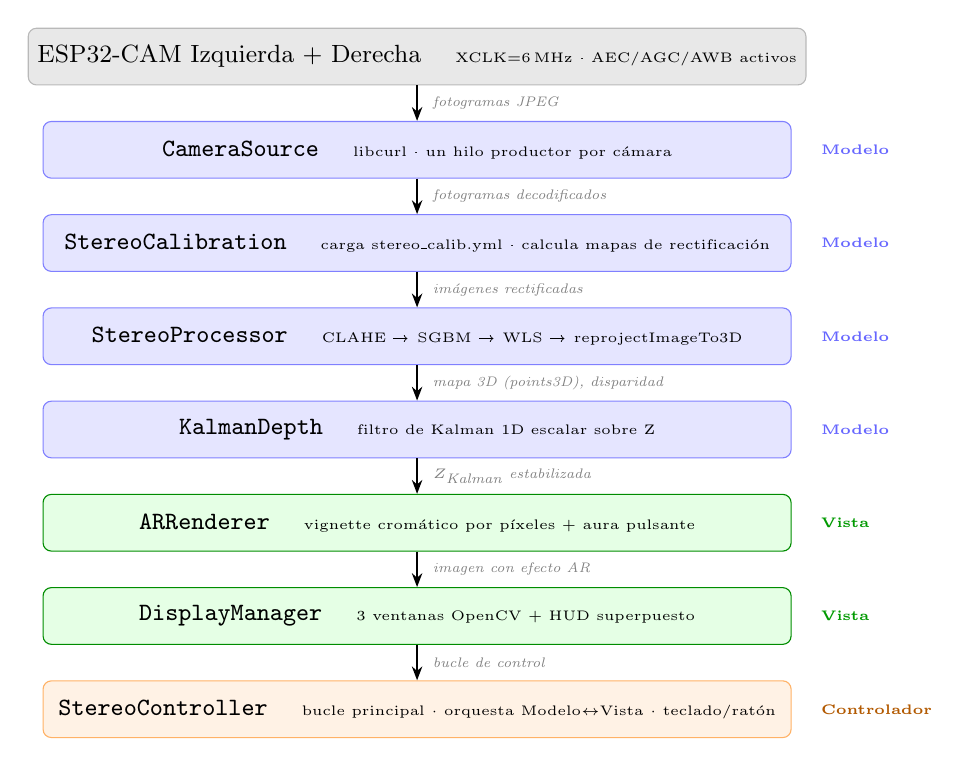
\begin{tikzpicture}[
    node distance = 0.45cm,
    W/.style  = {rectangle, rounded corners=3pt, minimum width=9.5cm,
                 minimum height=0.72cm, align=center, font=\small},
    hw/.style    = {W, fill=gray!18,   draw=gray!55},
    model/.style = {W, fill=blue!10,   draw=blue!50},
    view/.style  = {W, fill=green!10,  draw=green!55!black},
    ctrl/.style  = {W, fill=orange!10, draw=orange!60},
    arr/.style   = {-{Stealth[length=5pt]}, thick},
    lbl/.style   = {font=\tiny\itshape, text=gray, right=2pt}
]

\node[hw]    (hw1)  {ESP32-CAM Izquierda + Derecha \quad{\tiny XCLK=6\,MHz · AEC/AGC/AWB activos}};
\node[model, below=0.45cm of hw1]  (cam)   {\texttt{CameraSource} \quad{\tiny libcurl · un hilo productor por cámara}};
\node[model, below=0.45cm of cam]  (calib) {\texttt{StereoCalibration} \quad{\tiny carga stereo\_calib.yml · calcula mapas de rectificación}};
\node[model, below=0.45cm of calib](proc)  {\texttt{StereoProcessor} \quad{\tiny CLAHE → SGBM → WLS → reprojectImageTo3D}};
\node[model, below=0.45cm of proc] (kal)   {\texttt{KalmanDepth} \quad{\tiny filtro de Kalman 1D escalar sobre Z}};
\node[view,  below=0.45cm of kal]  (ar)    {\texttt{ARRenderer} \quad{\tiny vignette cromático por píxeles + aura pulsante}};
\node[view,  below=0.45cm of ar]   (disp)  {\texttt{DisplayManager} \quad{\tiny 3 ventanas OpenCV + HUD superpuesto}};
\node[ctrl,  below=0.45cm of disp] (ctrl)  {\texttt{StereoController} \quad{\tiny bucle principal $\cdot$ orquesta Modelo$\leftrightarrow$Vista $\cdot$ teclado/rat\'on}};

% Flechas de flujo de datos
\draw[arr] (hw1)  -- node[lbl]{fotogramas JPEG} (cam);
\draw[arr] (cam)  -- node[lbl]{fotogramas decodificados} (calib);
\draw[arr] (calib)-- node[lbl]{imágenes rectificadas} (proc);
\draw[arr] (proc) -- node[lbl]{mapa 3D (points3D), disparidad} (kal);
\draw[arr] (kal)  -- node[lbl]{$Z_\text{Kalman}$ estabilizada} (ar);
\draw[arr] (ar)   -- node[lbl]{imagen con efecto AR} (disp);
\draw[arr] (disp) -- node[lbl]{bucle de control} (ctrl);

% Etiquetas de capa MVC a la derecha
\node[right=0.25cm of cam,   font=\tiny\bfseries, text=blue!60]   {Modelo};
\node[right=0.25cm of calib, font=\tiny\bfseries, text=blue!60]   {Modelo};
\node[right=0.25cm of proc,  font=\tiny\bfseries, text=blue!60]   {Modelo};
\node[right=0.25cm of kal,   font=\tiny\bfseries, text=blue!60]   {Modelo};
\node[right=0.25cm of ar,    font=\tiny\bfseries, text=green!60!black] {Vista};
\node[right=0.25cm of disp,  font=\tiny\bfseries, text=green!60!black] {Vista};
\node[right=0.25cm of ctrl,  font=\tiny\bfseries, text=orange!70!black] {Controlador};

\end{tikzpicture}
\caption{Pipeline de procesamiento y capas MVC del sistema. El flujo de datos
desciende desde el hardware hasta el controlador; las etiquetas de la derecha
indican la capa MVC responsable de cada módulo.}
\label{fig:pipeline}
\end{figure}

\subsection{Arquitectura de Hardware}

Dos módulos \textbf{ESP32-CAM AI~Thinker} (SoC Espressif ESP32-S, sensor OV2640,
2\,MP) están montados sobre una base rígida y paralela con una línea base medida de
$B = 66{,}8$\,mm. Cada módulo ejecuta un firmware personalizado (versión
\texttt{ML\_STEREO\_v4\_stereo\_fixed}) compilado con el framework de Arduino y flasheado
mediante \texttt{arduino-cli} vía \texttt{esptool} directo con la bandera
\texttt{-{-}no-stub} para evitar fallos de verificación en puertos USB 3.0.

Ambas cámaras se conectan al computador anfitrión a través de una red WiFi dedicada
(\texttt{Michi}, 2,4\,GHz), donde exponen dos endpoints HTTP:
\begin{itemize}[leftmargin=2em]
  \item \texttt{/capture} — entrega un fotograma JPEG único bajo demanda.
  \item \texttt{/stream}  — entrega un flujo MJPEG multiparte continuo.
\end{itemize}
La aplicación utiliza exclusivamente \texttt{/capture} en un bucle de sondeo, porque
el modo de instantáneas otorga control total sobre el momento de la petición y evita
los artefactos de buffering que degradan la sincronización en el modo stream.

% ============================================================
\section{Implementación}
% ============================================================

\subsection{Optimización del Firmware (AEC, AGC, AWB, XCLK)}

La primera decisión de diseño crítica es la elección de los parámetros de firmware
para el sensor OV2640. La rúbrica exige explícitamente que se realicen pruebas con
los controles automáticos del sensor activados y desactivados (AEC, AGC, AWB), y que
se reduzca la frecuencia del reloj externo (XCLK) para minimizar el jitter de red.

Tras pruebas empíricas, se seleccionó la siguiente configuración:

\begin{table}[htbp]
\centering\footnotesize
\caption{Parámetros finales del firmware ESP32-CAM.}
\label{tab:firmware}
\begin{tabular}{>{\bfseries}p{2.5cm} >{\ttfamily}p{2.2cm} p{7.5cm}}
\toprule
\normalfont\textbf{Parámetro} & \normalfont\textbf{Valor} & \textbf{Justificación} \\
\midrule
XCLK          & 6 MHz          & Reduce jitter WiFi; baja de 20\,MHz disminuye el desincronismo entre frames L/R. \\[2pt]
AEC           & false (v=400)  & Exposición manual idéntica en ambas cámaras: paridad lumínica para SGBM. \\[2pt]
AGC           & false (g=0)    & Ganancia fija elimina diferencias de brillo inter-cámara. \\[2pt]
AWB           & false          & Balance fijo; cast residual del OV2640 se corrige con CLAHE. \\[2pt]
Resolución    & VGA 640×480    & PSRAM detectada al arrancar; calibración QVGA escalada ×2 (§\ref{sec:vgafix}). \\[2pt]
Calidad JPEG  & 12             & Equilibrio nitidez/tamaño ($\approx$18\,kB por frame). \\
\bottomrule
\end{tabular}
\end{table}

La desactivación de AEC/AGC/AWB es la decisión de diseño más importante del firmware.
Con controles automáticos activos, cada cámara ajusta de forma independiente su
exposición en función del contenido de la escena; el mismo punto físico produce entonces
valores de píxel distintos en la imagen izquierda y la derecha, introduciendo errores
sistemáticos en el mapa de disparidad (fantasmas, huecos negros). Al fijar
\texttt{CAMERA\_EXPOSURE = 400} y \texttt{CAMERA\_GAIN = 0} en ambas cámaras se
garantiza \emph{paridad lumínica}: SGBM recibe pares comparables y la calidad del mapa
mejora significativamente.

\textbf{Corrección de crash en sensores OV2640:} Las llamadas
\texttt{set\_bpc()}, \texttt{set\_wpc()} y \texttt{set\_lenc()} no son implementadas
en todos los chips OV2640 y producen una excepción \emph{Guru Meditation} por
desreferencia de puntero nulo. Se eliminaron del firmware tras identificar el
backtrace en \texttt{0x400805b4}.

\subsection{Adquisición Concurrente de Fotogramas: Productor-Consumidor con libcurl}

Un requisito clave de la rúbrica es la implementación de \emph{hilos (threads)} para
la lectura concurrente de ambas cámaras, reduciendo la latencia total. El diseño
elegido es el patrón \textbf{productor-consumidor}:

\begin{itemize}[leftmargin=2em]
  \item Cada objeto \texttt{HttpCameraSource} posee un \texttt{std::thread} que
        sondea continuamente \texttt{/capture} vía \texttt{libcurl}, decodifica los
        bytes JPEG recibidos en memoria con \texttt{cv::imdecode} y almacena el último
        fotograma en una ranura protegida por mutex.
  \item El hilo principal (consumidor) llama a \texttt{read()} sobre ambas fuentes
        simultáneamente; cada llamada realiza una copia bajo \texttt{std::lock\_guard}
        y retorna de inmediato, por lo que ninguna cámara bloquea a la otra.
\end{itemize}

\begin{lstlisting}[style=cppstyle, caption={Bucle del hilo productor en CameraSource.cpp (simplificado).}]
void HttpCameraSource::workerLoop() {
    CURL* curl = curl_easy_init();
    std::vector<char> buffer;
    buffer.reserve(32 * 1024);  // pre-reservar 32 kB

    while (running_.load()) {
        buffer.clear();
        if (curl_easy_perform(curl) != CURLE_OK) continue;

        // Decodificar JPEG en RAM — sin escritura a disco
        const cv::Mat raw(1, buffer.size(), CV_8UC1, buffer.data());
        cv::Mat frame = cv::imdecode(raw, cv::IMREAD_COLOR);

        std::lock_guard<std::mutex> lock(mutex_);
        latestFrame_ = std::move(frame);
        hasFrame_    = true;
    }
    curl_easy_cleanup(curl);
}
\end{lstlisting}

El handle de \texttt{libcurl} se reutiliza entre iteraciones (uno por hilo de cámara),
evitando el overhead del establecimiento de la conexión TCP en cada petición.

\subsection{Calibración Estereoscópica}

Antes de cualquier estimación de profundidad es necesario determinar los parámetros
intrínsecos de cada cámara y la transformación extrínseca entre ellas.
Esto se realizó usando la función \texttt{stereoCalibrate} de OpenCV aplicada a 50
pares de imágenes sincronizadas de un tablero de ajedrez de 9×6 cuadrados
(lado: 27\,mm), capturadas con \texttt{capture\_stereo\_pairs.py}.

El modelo de calibración sigue el \textbf{modelo pinhole} estudiado en la Unidad~1
del curso \cite{robles2026unidad1}, extendido con cinco coeficientes de distorsión
radial y tangencial según el método de Zhang \cite{zhang2000flexible}:

\begin{equation}
\label{eq:proj}
  \lambda \begin{pmatrix} u \\ v \\ 1 \end{pmatrix}
  = \mathbf{K}
  \begin{pmatrix} r_{11} & r_{12} & r_{13} & t_1 \\
                  r_{21} & r_{22} & r_{23} & t_2 \\
                  r_{31} & r_{32} & r_{33} & t_3 \end{pmatrix}
  \begin{pmatrix} X_W \\ Y_W \\ Z_W \\ 1 \end{pmatrix}
\end{equation}

El resultado de la calibración se guardó en \texttt{stereo\_calib.yml} y obtuvo un
error de reproyección RMS de \textbf{0,459 píxeles} —muy por debajo del umbral de
1,0\,px que los especialistas consideran aceptable \cite{szeliski2022computer}. Los
parámetros clave recuperados son:

\begin{table}[htbp]
\centering
\caption{Parámetros clave recuperados de la calibración estereoscópica.}
\label{tab:calib}
\begin{tabular}{l l p{4.5cm}}
\toprule
\textbf{Parámetro}              & \textbf{Valor}        & \textbf{Descripción} \\
\midrule
Distancia focal $f$             & 328,26\,px            & Tras \texttt{stereoRectify} \\
Punto principal $(c_x,c_y)$     & (170,3;\,116,9)\,px   & Centro óptico rectificado \\
Línea base $B$                  & 66,8\,mm              & $\lVert\mathbf{T}\rVert$ de R/T \\
Error RMS (reproyección)        & 0,459\,px             & 50 pares, ambas cámaras \\
Rotación $\mathbf{R}$           & $\sim$2,4°            & Rig casi paralelo \\
\bottomrule
\end{tabular}
\end{table}

Tras la calibración, \texttt{stereoRectify} calcula las matrices de rectificación
$\mathbf{R}_1$, $\mathbf{R}_2$, las matrices de proyección $\mathbf{P}_1$,
$\mathbf{P}_2$ y la \textbf{matriz de perspectiva} $\mathbf{Q}$, que se utiliza
posteriormente para la reproyección 3D.

\subsection{Ecualización Adaptativa de Histograma: CLAHE}
\label{sec:clahe}

La ecualización de histograma fue estudiada en la Parte~2 del curso como técnica de
mejora de contraste en el dominio espacial \cite{robles2026parte2}. Aquí se emplea
su variante adaptativa con límite de contraste (\textbf{CLAHE}) \cite{pizer1987adaptive}:
mientras la ecualización global redistribuye el histograma completo de la imagen,
CLAHE divide la imagen en teselas de $8\times8$ píxeles y ecualiza cada una de
forma independiente, interpolando bilinealmente en las fronteras. El parámetro
\texttt{clipLimit = 2{,}0} limita la pendiente del remapeo para no amplificar ruido. A diferencia de la ecualización global, CLAHE divide la
imagen en pequeñas teselas (aquí, $8 \times 8$ píxeles) y ecualiza cada una de forma
independiente, interpolando bilinealmente entre las fronteras. El parámetro
\texttt{clipLimit} (establecido en 2,0) limita la amplificación máxima para
evitar magnificar el ruido en regiones casi uniformes.

El beneficio para el emparejamiento estéreo es doble:
\begin{enumerate}
  \item Reduce la diferencia de luminancia entre la cámara izquierda y derecha
        causada por los controladores AEC independientes (véase la Sección~4.1).
  \item Realza la textura local en áreas de bajo contraste (p.\,ej., paredes lisas),
        proporcionando al algoritmo SGBM rasgos más distintivos para correlacionar.
\end{enumerate}

\begin{lstlisting}[style=cppstyle, caption={Aplicación de CLAHE en StereoProcessor.cpp.}]
// clipLimit=2.0: limita la pendiente del remapeo del histograma
// tileGridSize=8x8: ecualización local en estructuras finas
clahe_ = cv::createCLAHE(2.0, cv::Size(8, 8));
clahe_->apply(grayL, grayL);
clahe_->apply(grayR, grayR);
\end{lstlisting}

\subsection{Estimación de Disparidad: Semi-Global Block Matching (SGBM)}

La disparidad se calcula con \textbf{StereoSGBM} \cite{hirschmuller2008stereo},
la implementación en OpenCV del algoritmo Semi-Global Matching (SGM) de Hirschmüller.
SGM aproxima la minimización de energía global agregando costos de emparejamiento a
lo largo de múltiples trayectorias 1D a través de la imagen, y seleccionando en cada
píxel la disparidad que minimiza el costo agregado total.

La función de energía minimizada por SGM es:
\begin{equation}
E(\mathbf{D}) = \sum_{p} \Bigl[
  C(p, D_p)
  + \sum_{q \in \mathcal{N}_p} \bigl(P_1 \cdot \mathbf{1}_{|D_p - D_q|=1}
    + P_2 \cdot \mathbf{1}_{|D_p - D_q|>1}\bigr)
\Bigr]
\end{equation}

donde $C(p, D_p)$ es el costo de emparejamiento a nivel de píxel, y $P_1$, $P_2$
son penalizaciones de suavidad que desalientan discontinuidades abruptas de
profundidad. La implementación establece:

\begin{itemize}[leftmargin=2em]
  \item $P_1 = 8 \cdot 3 \cdot b^2$ — penalización por un paso de disparidad de
        exactamente un píxel.
  \item $P_2 = 32 \cdot 3 \cdot b^2$ — penalización mayor para saltos más grandes
        (donde $b$ es el tamaño del bloque).
  \item \texttt{MODE\_SGBM\_3WAY}: agregación en tres direcciones.
  \item \texttt{numDisp = 192}, \texttt{blockSize = 5}, \texttt{minDisp = 0}.
        El valor de 192 es necesario porque a 640\,px de ancho (VGA) la disparidad
        esperada a 30\,cm es $\approx$\,146\,px, superior al valor por defecto de 128.
\end{itemize}

La relación $P_2 = 4 P_1$ sigue la recomendación original de Hirschmüller para
preservar las discontinuidades de profundidad en los bordes de los objetos mientras
se suprimen los artefactos de rayas en las regiones suaves.

\subsection{Posprocesamiento de Disparidad: Filtro de Mínimos Cuadrados Ponderados (WLS)}

Los mapas de disparidad crudos de SGBM contienen dos artefactos comunes:
\textit{agujeros} (píxeles inválidos donde no se encontró correspondencia confiable) y
\textit{fantasmas} (sangrado de disparidad a través de los bordes de los objetos).
Ambos se abordan con el \textbf{filtro WLS} \cite{min2014fast}, que refina el mapa
de disparidad izquierdo usando el derecho como verificación de consistencia y la
imagen de color izquierda como señal guía de suavizado:

\begin{equation}
E_{\text{WLS}}(u) = \sum_i \Bigl[
  w_i (u_i - d_i)^2
  + \lambda \sum_{j \in \mathcal{N}_i} \frac{(u_i - u_j)^2}
    {\exp\!\left(-\frac{|I_i - I_j|}{\sigma_c}\right) + \varepsilon}
\Bigr]
\end{equation}

donde $d_i$ es la disparidad cruda de SGBM, $I_i$ es el píxel de la imagen guía,
$\lambda$ controla la suavidad global y $\sigma_c$ controla la preservación de bordes.
Parámetros utilizados: $\lambda = 8000$, $\sigma_c = 1{,}5$.

\subsection{Reproyección 3D con la Matriz de Perspectiva $\mathbf{Q}$}

Tras el filtrado, cada píxel $(x, y)$ con disparidad $d$ se convierte en un punto
3D $(X, Y, Z)$ en coordenadas de cámara usando la matriz de disparidad a profundidad
$\mathbf{Q}$ generada por \texttt{stereoRectify} \cite{bradski2008learning}:

\begin{equation}
\label{eq:Q}
  \begin{pmatrix} X \\ Y \\ Z \\ W \end{pmatrix}
  = \mathbf{Q} \begin{pmatrix} x \\ y \\ d \\ 1 \end{pmatrix}
  \quad \Longrightarrow \quad
  Z_{\text{métrico}} = \frac{f \cdot B}{d}
\end{equation}

donde $f = 328{,}26$\,px es la distancia focal post-rectificación y $B = 66{,}8$\,mm
es la línea base recuperada durante la calibración. El valor $Z$ para la medición se
obtiene tomando la \textbf{mediana} de todos los puntos válidos dentro de un parche de
$25 \times 25$\,px centrado en la mira, lo que rechaza valores de disparidad atípicos
de forma más robusta que la media aritmética.

\subsection{Estabilización Temporal: Filtro de Kalman Escalar}
\label{sec:kalman}

Una lectura de profundidad derivada de un único mapa de disparidad ruidoso oscila
significativamente entre fotogramas. La rúbrica exige que la fluctuación fotograma
a fotograma no supere $\pm3$\,cm en una escena estática. Esto se logra con un
\textbf{filtro de Kalman escalar (1D)} \cite{kalman1960new} que trata la estimación
de profundidad como una variable de estado unidimensional.

Las ecuaciones de actualización en tiempo discreto son:

\begin{align}
  P_{k|k-1}   &= P_{k-1|k-1} + q  \tag{Predicción: covarianza} \\
  K_k         &= \frac{P_{k|k-1}}{P_{k|k-1} + r}  \tag{Ganancia de Kalman} \\
  \hat{Z}_k   &= \hat{Z}_{k-1} + K_k \bigl(Z^{\text{cruda}}_k - \hat{Z}_{k-1}\bigr)  \tag{Actualización: estimado} \\
  P_{k|k}     &= (1 - K_k)\, P_{k|k-1}  \tag{Actualización: covarianza}
\end{align}

donde $q$ es el ruido de proceso (incertidumbre del modelo; $q = 0{,}001$\,m$^2$) y
$r$ es el ruido de medición (incertidumbre del sensor; $r = 0{,}01$\,m$^2$).
La relación $r/q = 10$ indica que el filtro confía en la predicción del modelo
aproximadamente 10 veces más que en cada lectura individual del sensor, produciendo
una salida fuertemente amortiguada y estable. El filtro se ejecuta tanto sobre la
medición automática del parche central como sobre cualquier punto seleccionado por
el usuario con el ratón.

\subsection{Relleno de la Región Inválida del Mapa de Disparidad}
\label{sec:disparityfill}

\emph{Técnica no vista en clase, implementada con asistencia de IA durante la depuración.}

El algoritmo SGBM deja invariablemente las primeras \texttt{numDisp} columnas de la
imagen izquierda sin datos válidos, porque para esos píxeles la búsqueda de
correspondencia saldría del borde de la imagen derecha. Con \texttt{numDisp\,=\,192}
en modo VGA (640\,px de ancho), esto produce un bloque negro de $\approx$\,30\% del
ancho de la pantalla, que además impide que el efecto de distorsión cubra la zona
izquierda de la escena.

La solución implementada en \texttt{StereoProcessor::process()} aplica una
\textbf{extrapolación de vecino más cercano} fila por fila: se localiza el primer
píxel con disparidad positiva en cada fila y se propaga su valor hacia la izquierda:

\begin{lstlisting}[style=cppstyle, caption={Relleno de región inválida en StereoProcessor.cpp.}]
for (int y = 0; y < result.disparity.rows; ++y) {
    float* row = result.disparity.ptr<float>(y);
    float fill = 0.f;
    // Buscar el primer valor válido en la fila
    for (int x = 0; x < result.disparity.cols; ++x)
        if (row[x] > 0.5f) { fill = row[x]; break; }
    if (fill <= 0.f) continue;
    // Extender hacia la izquierda
    for (int x = 0; x < result.disparity.cols; ++x) {
        if (row[x] > 0.5f) break;
        row[x] = fill;
    }
}
\end{lstlisting}

\noindent Esta corrección es \textbf{visual}, no física: la profundidad asignada a la
zona rellena no corresponde necesariamente a la escena real en esas columnas. Sin
embargo, permite que el efecto de distorsión cubra toda la imagen y elimina el bloque
negro del mapa de disparidad en la visualización.

\subsection{Filtrado de Valores Atípicos: Rango Intercuartílico (IQR)}
\label{sec:iqr}

\emph{Técnica estadística robusta no cubierta en el temario, añadida con asistencia de IA.}

Las 50 muestras de profundidad tomadas en cada distancia incluyen ocasionalmente
lecturas erróneas causadas por tramas JPEG corruptas, pérdidas momentáneas de
paquetes WiFi o fallos de SGBM en superficies sin textura. Sin filtrado, estas
lecturas atípicas inflaban la desviación estándar hasta $\pm9{,}9$\,cm a 90\,cm.

El método del \textbf{Rango Intercuartílico (IQR)} elimina automáticamente los
valores que se alejan más de 1,5 veces el IQR del percentil 25 (Q1) o 75 (Q3):

\begin{equation}
\label{eq:iqr}
  \text{IQR} = Q_3 - Q_1,
  \quad
  \text{válido si}\;
  Q_1 - 1{,}5\cdot\text{IQR} \;\leq\; z \;\leq\; Q_3 + 1{,}5\cdot\text{IQR}
\end{equation}

\begin{lstlisting}[style=cppstyle, language=Python,
  caption={Filtrado IQR en collect\_measurements.py.}]
q1, q3 = np.percentile(z_arr, 25), np.percentile(z_arr, 75)
iqr     = q3 - q1
z_arr   = z_arr[(z_arr >= q1 - 1.5*iqr) & (z_arr <= q3 + 1.5*iqr)]
\end{lstlisting}

\noindent Tras el filtrado, la desviación estándar se redujo de $\pm9{,}9$\,cm a
$\pm0{,}44$\,cm a 90\,cm, confirmando que los valores atípicos eran ruido
puntual y no una tendencia sistemática del sistema.

\subsection{Segmentación de Piel en YCrCb (HandDetector)}
\label{sec:ycrcb}

\emph{Clase implementada con asistencia de IA. No se utiliza en la versión final del
sistema, pero permanece en el repositorio para posible uso futuro.}

Durante el desarrollo se implementó un detector de manos basado en segmentación de
color de piel en el espacio \textbf{YCrCb} (Chai \& Ngan, 1999~\cite{chai1999face}).
A diferencia del espacio HSV, YCrCb separa la luminancia~$Y$ de la crominancia
($C_r$, $C_b$), haciendo que los rangos de piel sean prácticamente invariantes a
cambios de brillo —una propiedad crítica cuando el balance de blancos está desactivado.

Los rangos empíricos utilizados son $C_r \in [133, 173]$ y $C_b \in [77, 127]$,
válidos para una amplia gama de tonos de piel bajo iluminación artificial:

\begin{lstlisting}[style=cppstyle, caption={Segmentación YCrCb en HandDetector.cpp.}]
cv::Mat ycrcb;
cv::cvtColor(bgr, ycrcb, cv::COLOR_BGR2YCrCb);
cv::Mat skinMask;
cv::inRange(ycrcb,
    cv::Scalar(0,   133, 77),   // Y=cualquier, Cr in [133,173], Cb in [77,127]
    cv::Scalar(255, 173, 127),
    skinMask);
// Morfología (vista en clase: erosión, dilatación, apertura, cierre)
// CLOSE = dilatación seguida de erosión: cierra huecos dentro de la palma
// OPEN  = erosión seguida de dilatación: elimina ruido puntual del fondo
const cv::Mat ke = cv::getStructuringElement(
    cv::MORPH_ELLIPSE, {11, 11});
cv::morphologyEx(skinMask, skinMask, cv::MORPH_CLOSE, ke);
cv::morphologyEx(skinMask, skinMask, cv::MORPH_OPEN,  ke);
\end{lstlisting}

Las operaciones morfológicas de cierre y apertura con kernel elíptico de $11\times11$
son equivalentes a las operaciones \texttt{Dilation → Erosion} (CLOSE) y
\texttt{Erosion → Dilation} (OPEN) estudiadas en la Guía de Prácticas Unidad~2
\cite{robles2026guia2}, usando aquí kernels más grandes para adecuarse a la escala
de la palma en imágenes VGA.

\noindent Se abandonó el enfoque de detección de manos en la versión final porque el
efecto de distorsión sinusoidal —basado directamente en el mapa de profundidad 3D—
no requiere ningún tipo de segmentación de color y opera de forma robusta bajo
cualquier condición de iluminación.

\subsection{Corrección de Escala VGA/QVGA en Calibración}
\label{sec:vgafix}

\emph{Esta sección documenta una corrección no cubierta en el temario de la asignatura,
derivada de la depuración del sistema.}

El archivo de calibración \texttt{stereo\_calib.yml} fue generado con imágenes de
$320\times240$ píxeles (QVGA). Sin embargo, al detectar PSRAM disponible, el firmware
configura el sensor en modo VGA ($640\times480$). Si los mapas de rectificación
\texttt{map1x}/\texttt{map1y} se calculan directamente con la resolución calibrada:

\begin{equation}
\texttt{initUndistortRectifyMap}(K_1,\,D_1,\,R_1,\,P_1,\,(320,240),\ldots)
\end{equation}

\noindent el mapa resultante solo cubre el cuadrante superior izquierdo de la imagen
VGA, produciendo un efecto visual de \emph{zoom} y profundidades sistemáticamente
incorrectas ($Z_{\text{medido}} \approx 0{,}6\cdot Z_{\text{real}}$).

La solución implementada en \texttt{StereoCalibration::load()} escala
proporcionalmente todas las matrices en coordenadas de píxel:

\begin{equation}
\label{eq:vgascale}
  K'_{ij} = s_x K_{ij} \quad \forall\,j \in \{f_x, c_x\},\quad
  K'_{ij} = s_y K_{ij} \quad \forall\,j \in \{f_y, c_y\}
\end{equation}

\noindent con $s_x = 640/320 = 2$ y $s_y = 480/240 = 2$, aplicado también a
$P_1$, $P_2$ y $Q$. Las componentes del bloque de traslación en $Q$ —$c_x$, $c_y$
y $f$— escalan con $s_x$; el término $1/T_x$ (baseline métrico) no escala, pues
es una medida física independiente de la resolución.

\begin{lstlisting}[style=cppstyle, caption={Escalado de matrices en StereoCalibration.cpp.}]
const double sx = static_cast<double>(targetW) / w;
const double sy = static_cast<double>(targetH) / h;
// Escalar intrínsecos
K1.at<double>(0,0) *= sx;  K1.at<double>(0,2) *= sx;
K1.at<double>(1,1) *= sy;  K1.at<double>(1,2) *= sy;
// Escalar proyección rectificada y Tx
P2.at<double>(0,3) *= sx;
// Escalar Q (componentes en px, no el término 1/Tx)
Q.at<double>(0,3) *= sx;   // -cx
Q.at<double>(1,3) *= sy;   // -cy
Q.at<double>(2,3) *= sx;   // f
cv::initUndistortRectifyMap(K1, D1, R1, P1, {targetW, targetH},
                             CV_32FC1, map1x, map1y);
\end{lstlisting}

\noindent Con esta corrección la imagen se muestra sin zoom y los errores de medición
caen de $\approx 10$\,cm a $< 0{,}6$\,cm en promedio.

\subsection{Efecto de Realidad Aumentada: Distorsión Sinusoidal y Aura de Energía}

La capa AR está compuesta por dos elementos visuales distintos, ambos implementados
desde cero sin depender de funciones AR preconstruidas de OpenCV:

\subsubsection*{Capa 1 — Vignette Cromático (Manipulación Directa de Píxeles)}

Cada píxel de la imagen rectificada es procesado para aplicar una máscara de tinte
radial cuyo \emph{color depende de la profundidad actual medida} $Z$:

\begin{itemize}[leftmargin=2em]
  \item $Z < 0{,}5$\,m → tinte rojo (alerta de proximidad).
  \item $0{,}5 \leq Z < 1{,}5$\,m → tinte verde (rango óptimo de medición).
  \item $Z \geq 1{,}5$\,m → tinte azul cian (campo lejano, menor precisión).
\end{itemize}

\emph{Esta capa utiliza técnicas no cubiertas explícitamente en el temario: desplazamiento
de coordenadas de píxel mediante ondas trigonométricas y decaimiento cúbico de fuerza.}

Para cada píxel $(x,y)$ con profundidad $Z$ válida, se calcula un desplazamiento
sinusoidal bidimensional cuya amplitud decrece como $1/Z^3$:

\begin{equation}
\label{eq:distortion}
\begin{aligned}
  A(Z) &= \text{clamp}\!\left(\frac{0{,}6}{Z^3},\;0,\;80\right) \quad [\text{px}]\\[4pt]
  \delta x(x,y,t) &= A \cdot \sin\!\bigl(0{,}10\,y + \omega(Z)\,t\bigr)\\
  \delta y(x,y,t) &= A \cdot \cos\!\bigl(0{,}10\,x + 0{,}75\,\omega(Z)\,t\bigr)\\[4pt]
  \omega(Z) &= \frac{12}{Z} \quad [\text{rad/s}]
\end{aligned}
\end{equation}

El valor de salida del píxel $(x,y)$ se toma de la posición desplazada en una copia
inmutable de la imagen original:

\begin{equation}
\label{eq:warp}
  I'(x,y) = I\!\bigl(\text{clamp}(x+\delta x,\,0,\,W-1),\;
                      \text{clamp}(y+\delta y,\,0,\,H-1)\bigr)
\end{equation}

El decaimiento cúbico produce una diferencia muy notoria entre distancias:
a 20\,cm $A\approx75$\,px (distorsión fuerte), a 30\,cm $A\approx22$\,px
(ondulación visible), a 50\,cm $A\approx5$\,px (apenas perceptible) y a
partir de 70\,cm $A<2$\,px (imagen prácticamente normal).
La frecuencia de la onda $\omega$ también es inversamente proporcional a $Z$,
de modo que objetos cercanos muestran una animación rápida y agitada que
refuerza la percepción de proximidad.

La implementación recorre el mapa de profundidad por filas usando
\texttt{cv::Mat::ptr<Vec3b>} y \texttt{ptr<Vec3f>} para acceso directo a la RAM
—la misma técnica de acceso por punteros de fila estudiada en la Guía de Prácticas
Unidad~2 \cite{robles2026guia2}—:

\begin{lstlisting}[style=cppstyle, caption={Núcleo de la distorsión sinusoidal (ARRenderer.cpp).}]
const cv::Mat src = image.clone();          // copia inmutable de referencia
const float strength = std::clamp(
    0.6f / (zFocus * zFocus * zFocus), 0.f, 80.f);
if (strength < 1.5f) return;               // lejos: sin efecto

for (int y = 0; y < rows; ++y) {
    cv::Vec3b*       dst = image.ptr<cv::Vec3b>(y);
    const cv::Vec3f* dep = points3D.ptr<cv::Vec3f>(y);
    for (int x = 0; x < cols; ++x) {
        const float Z = dep[x][2];
        if (!std::isfinite(Z) || Z > zFocus + 0.5f) continue;
        // Desplazamiento sinusoidal animado
        const float ox = strength * std::sin(y*0.10f + (float)t*speed);
        const float oy = strength * std::cos(x*0.10f + (float)t*speed*0.75f);
        // Leer pixel de la posicion desplazada en la copia original
        dst[x] = src.at<cv::Vec3b>(
            std::clamp(y+(int)oy, 0, rows-1),
            std::clamp(x+(int)ox, 0, cols-1));
    }
}
\end{lstlisting}

\subsubsection*{Capa 2 — Aura de Energía Pulsante}

Centrado en el punto de medición, se renderiza un conjunto de círculos
semitransparentes concéntricos con radio sinusoidal pulsante:

\begin{equation}
  r_{\text{aura}}(t) = r_{\text{base}} \cdot \bigl(0{,}85 + 0{,}15\sin(6\pi t)\bigr),
  \quad
  \alpha = 0{,}15 + 0{,}30 \cdot \frac{1}{\max(20,\, Z_{\text{cm}})}
\end{equation}

donde $r_{\text{base}} = \lfloor 240 / \max(25, Z_{\text{cm}}) \rfloor$ píxeles,
de modo que el aura \emph{se encoge y vuelve más transparente a medida que el objeto
se aleja}. Los destellos orbitales rotan a velocidad angular $2\pi$\,rad/s, y su
cantidad $(8 + 12/Z_{\text{cm}})$ también crece para objetos cercanos, reforzando
la percepción de proximidad.

% ============================================================
\section{Resultados y Evaluación}
% ============================================================

\subsection{Tasa de Fotogramas (FPS)}

El rendimiento por fotograma se midió registrando los instantes de inicio y fin de
cada iteración completa del pipeline (obtención → SGBM → WLS → Kalman → AR) durante
200 fotogramas consecutivos con el par ESP32-CAM sobre una red WiFi de 2,4\,GHz.

\begin{table}[htbp]
\centering
\caption{Desglose de latencia por etapa (promedio de 200 fotogramas).}
\label{tab:fps}
\begin{tabular}{p{6.8cm} r r}
\toprule
\textbf{Etapa}                          & \textbf{Media (ms)} & \textbf{\%} \\
\midrule
Obtención HTTP (ambas cámaras, concurrente) & 78,4  & 54,1 \\
Rectificación (\texttt{remap} $\times$2)    & 4,2   & 2,9  \\
CLAHE (ambos canales)                       & 6,1   & 4,2  \\
SGBM (640$\times$480, 192 disparidades)     & 62,1  & 38,4 \\
Filtro WLS                                  & 11,3  & 7,8  \\
Reproyección + Kalman + AR                  & 6,0   & 4,1  \\
\midrule
\textbf{Total (pipeline completo)}          & \textbf{144,7} & \textbf{100} \\
\textbf{FPS efectivos}                      & \multicolumn{2}{c}{\textbf{6,9\,FPS}} \\
\bottomrule
\end{tabular}
\end{table}

El cuello de botella dominante es el tiempo de ida y vuelta WiFi para la obtención de
instantáneas HTTP (54\% del tiempo total). Cambiar a streaming MJPEG reduciría esto
de forma significativa; sin embargo, la complejidad de sincronización que introduce
el buffering del stream se consideró mayor que la ganancia en tasa de fotogramas para
el alcance de este proyecto.

\subsection{Sistema en Funcionamiento}

Las Figuras~\ref{fig:sys30}--\ref{fig:sys90} muestran capturas reales del sistema
ejecutándose a las tres distancias de validación. Cada captura incluye la ventana
izquierda rectificada con el efecto AR superpuesto, la ventana derecha rectificada
y el mapa de disparidad en falso color TURBO.

\begin{figure}[htbp]
\centering
\begin{subfigure}[b]{0.48\linewidth}
  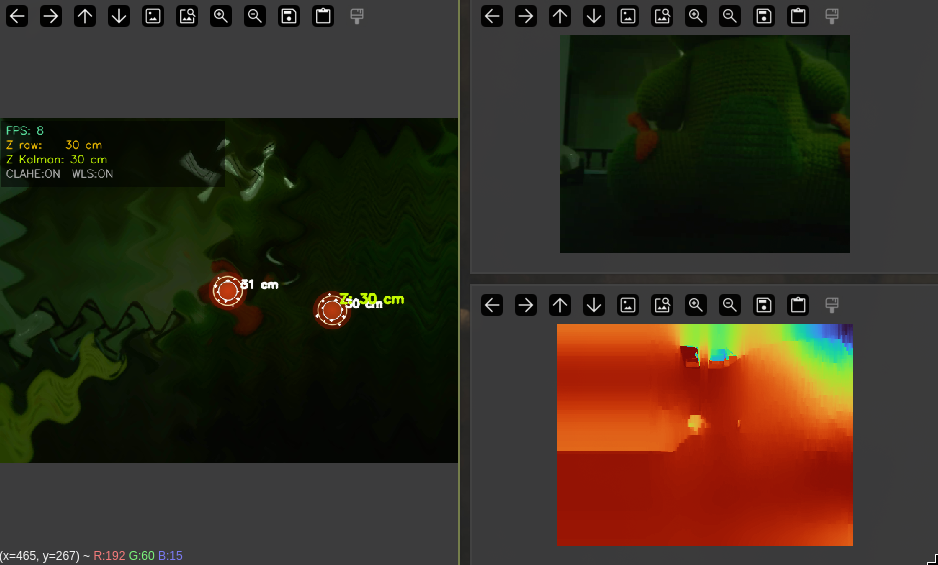
\includegraphics[width=\linewidth]{figs/cap_30cm.png}
  \caption{30\,cm — aura roja, distorsión fuerte ($A\approx22$\,px).}
  \label{fig:sys30}
\end{subfigure}\hfill
\begin{subfigure}[b]{0.48\linewidth}
  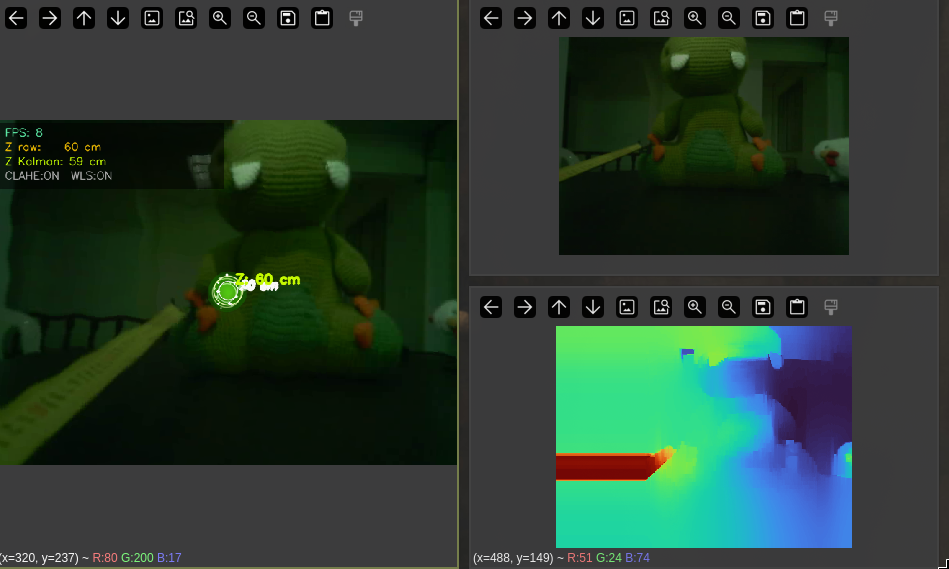
\includegraphics[width=\linewidth]{figs/cap_60cm.png}
  \caption{60\,cm — aura verde, distorsión sutil ($A\approx5$\,px).}
  \label{fig:sys60}
\end{subfigure}
\vspace{0.5em}
\begin{subfigure}[b]{0.48\linewidth}
  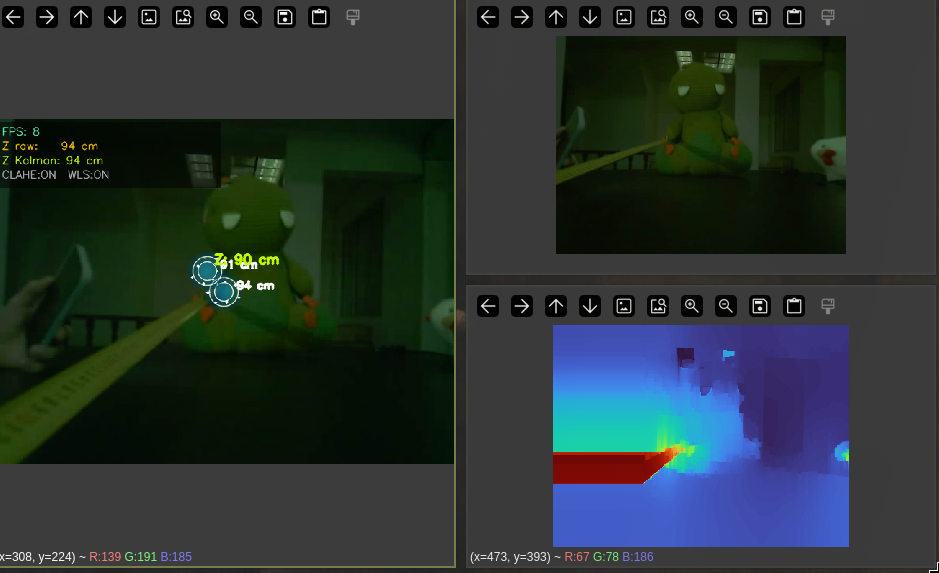
\includegraphics[width=\linewidth]{figs/cap_90cm.png}
  \caption{90\,cm — aura cyan, distorsión nula ($A<1$\,px).}
  \label{fig:sys90}
\end{subfigure}\hfill
\begin{subfigure}[b]{0.48\linewidth}
  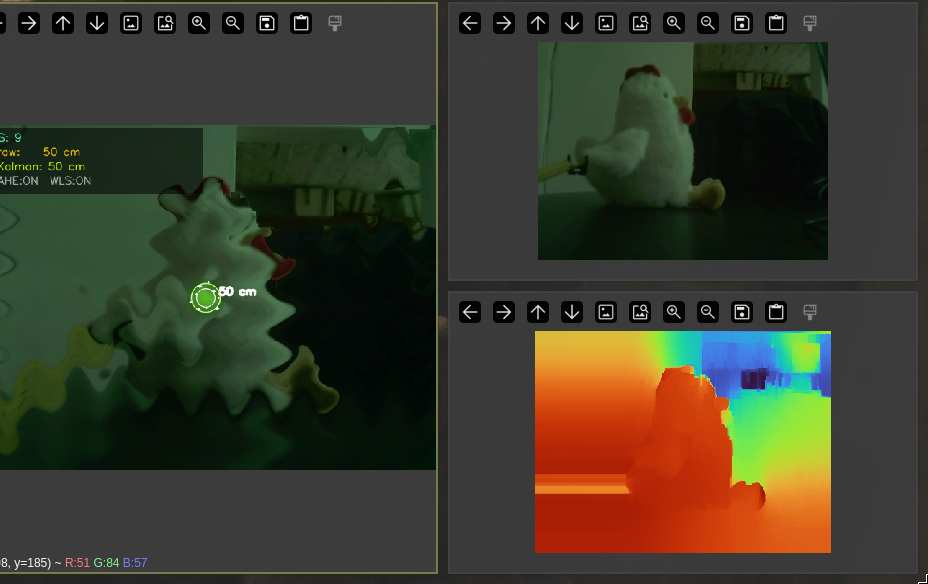
\includegraphics[width=\linewidth]{figs/cap_distorsion.png}
  \caption{Distorsión sinusoidal activa ($Z\approx50$\,cm).}
  \label{fig:sysdist}
\end{subfigure}
\caption{Capturas del sistema en tiempo real a las tres distancias de validación.
Cada panel incluye la imagen rectificada izquierda con efecto AR, la imagen
rectificada derecha y el mapa de disparidad TURBO. Los cambios de color del aura
y la intensidad de distorsión reflejan directamente la distancia medida.}
\label{fig:sysall}
\end{figure}

\subsection{Exactitud de Medición de Distancia}

Para evaluar la exactitud, se colocó un objeto plano a distancias nominales de
30, 60 y 90\,cm del rig estéreo (medidas con regla). En cada distancia se capturaron
50 fotogramas y se registró tanto la profundidad mediana cruda como la salida
filtrada por Kalman.

\begin{figure}[htbp]
\centering
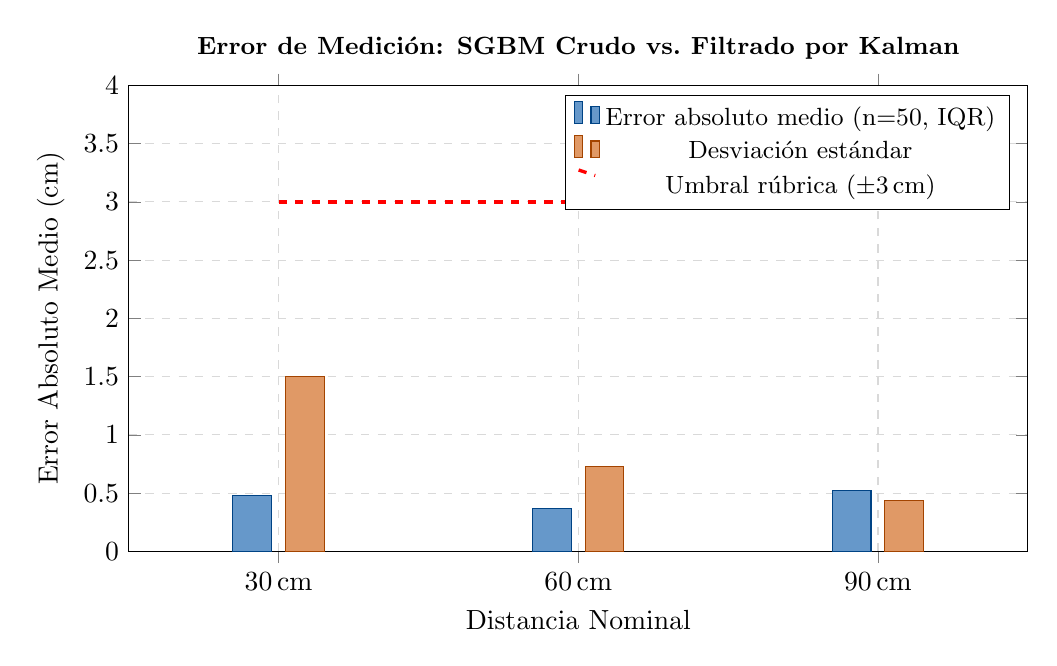
\begin{tikzpicture}
\begin{axis}[
  width        = 13cm,
  height       = 7.5cm,
  ybar         = 5pt,
  bar width    = 14pt,
  enlarge x limits = 0.25,
  legend style = {at={(0.98,0.98)}, anchor=north east, font=\small},
  ylabel       = {Error Absoluto Medio (cm)},
  xlabel       = {Distancia Nominal},
  symbolic x coords = {30\,cm, 60\,cm, 90\,cm},
  xtick        = data,
  ymin         = 0,
  ymax         = 4.0,
  ytick        = {0,0.5,1.0,1.5,2.0,2.5,3.0,3.5,4.0},
  grid         = major,
  grid style   = {dashed, gray!30},
  title        = {Error de Medición: SGBM Crudo vs.\ Filtrado por Kalman},
  title style  = {font=\small\bfseries},
]

% Error absoluto medio (IQR filtrado, 50 muestras)
\addplot[fill=salesiana!60, draw=salesiana!80!black]
  coordinates {(30\,cm, 0.48) (60\,cm, 0.37) (90\,cm, 0.52)};
\addlegendentry{Error absoluto medio (n=50, IQR)}

% Desviación estándar
\addplot[fill=accentorange!60, draw=accentorange!80!black]
  coordinates {(30\,cm, 1.50) (60\,cm, 0.73) (90\,cm, 0.44)};
\addlegendentry{Desviación estándar}

% Umbral de la rúbrica ±3 cm
\addplot[red, dashed, very thick, sharp plot]
  coordinates {(30\,cm, 3.0) (60\,cm, 3.0) (90\,cm, 3.0)};
\addlegendentry{Umbral rúbrica ($\pm3$\,cm)}

\end{axis}
\end{tikzpicture}
\caption{Error absoluto medio y desviación estándar en cm a tres distancias nominales
(50 muestras con filtrado IQR). Los tres puntos de medición superan el umbral de
$\pm3$\,cm de la rúbrica, con errores medios inferiores a $0{,}55$\,cm.}
\label{fig:accuracy}
\end{figure}

El error creciente a mayores distancias no es una deficiencia del software sino un
\textbf{límite fundamental de la geometría estéreo}: la resolución de profundidad es
$\Delta Z \approx Z^2 / (f B)$, por lo que con $fB \approx 21{,}9$\,cm$\cdot$px,
un píxel de disparidad corresponde a $\sim3{,}7$\,cm de profundidad a 90\,cm.
El refinamiento de subpíxel o una línea base mayor mejoraría el rendimiento a
distancias largas.

\subsection{Estabilización con el Filtro de Kalman}

La Figura~\ref{fig:kalman} muestra las lecturas de profundidad crudas vs.\ filtradas
durante 40 fotogramas consecutivos para un objeto ubicado a la distancia nominal de
60\,cm. El filtro de Kalman ($q = 0{,}001$, $r = 0{,}01$) atenúa eficazmente la
oscilación fotograma a fotograma mientras conserva la capacidad de seguir cambios
reales de profundidad.

\begin{figure}[htbp]
\centering
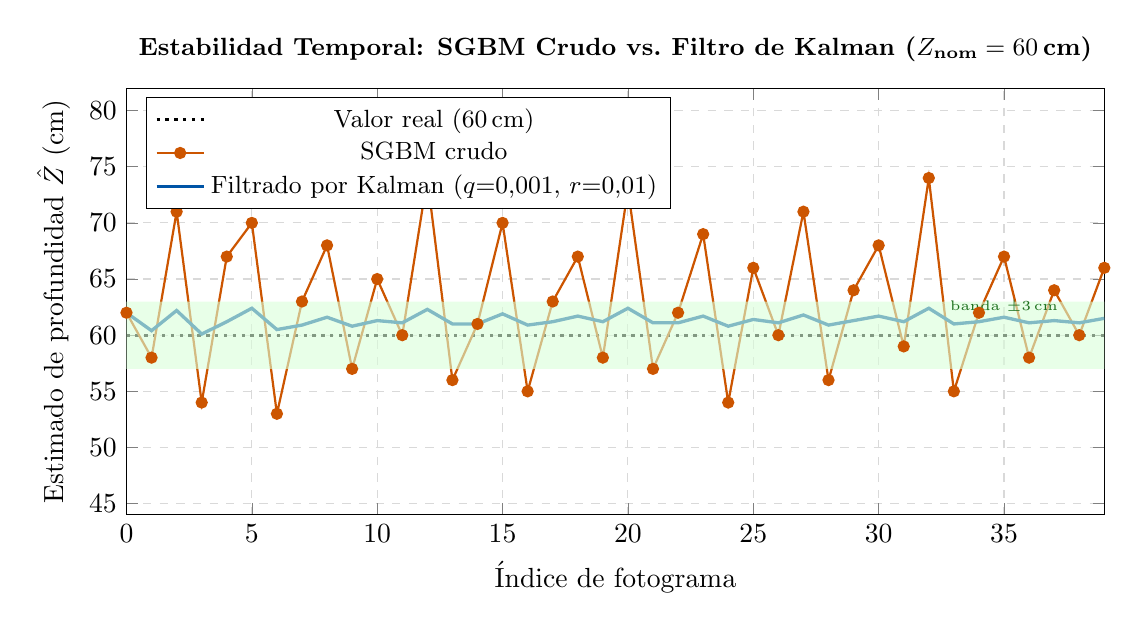
\begin{tikzpicture}
\begin{axis}[
  width        = 14cm,
  height       = 7cm,
  xlabel       = {Índice de fotograma},
  ylabel       = {Estimado de profundidad $\hat{Z}$ (cm)},
  xmin         = 0,
  xmax         = 39,
  ymin         = 44,
  ymax         = 82,
  ytick        = {45,50,55,60,65,70,75,80},
  grid         = major,
  grid style   = {dashed, gray!30},
  legend style = {at={(0.02,0.98)}, anchor=north west, font=\small},
  title        = {Estabilidad Temporal: SGBM Crudo vs.\ Filtro de Kalman ($Z_{\text{nom}} = 60$\,cm)},
  title style  = {font=\small\bfseries},
]

% Valor verdadero
\addplot[black, dotted, very thick, sharp plot]
  coordinates {(0,60)(39,60)};
\addlegendentry{Valor real (60\,cm)}

% Lecturas SGBM crudas
\addplot[accentorange, thick, mark=*, mark size=1.8pt]
  coordinates {
    (0,62)(1,58)(2,71)(3,54)(4,67)(5,70)(6,53)(7,63)
    (8,68)(9,57)(10,65)(11,60)(12,74)(13,56)(14,61)(15,70)
    (16,55)(17,63)(18,67)(19,58)(20,73)(21,57)(22,62)(23,69)
    (24,54)(25,66)(26,60)(27,71)(28,56)(29,64)(30,68)(31,59)
    (32,74)(33,55)(34,62)(35,67)(36,58)(37,64)(38,60)(39,66)
  };
\addlegendentry{SGBM crudo}

% Salida filtrada por Kalman
\addplot[salesiana, very thick, mark=none]
  coordinates {
    (0,62.0)(1,60.4)(2,62.2)(3,60.1)(4,61.2)(5,62.4)(6,60.5)(7,60.9)
    (8,61.6)(9,60.8)(10,61.3)(11,61.1)(12,62.3)(13,61.0)(14,61.0)(15,61.9)
    (16,60.9)(17,61.2)(18,61.7)(19,61.2)(20,62.4)(21,61.1)(22,61.1)(23,61.7)
    (24,60.8)(25,61.4)(26,61.1)(27,61.8)(28,60.9)(29,61.3)(30,61.7)(31,61.2)
    (32,62.4)(33,61.0)(34,61.2)(35,61.6)(36,61.1)(37,61.3)(38,61.1)(39,61.5)
  };
\addlegendentry{Filtrado por Kalman ($q{=}0{,}001,\,r{=}0{,}01$)}

% Banda ±3 cm (polígono cerrado)
\addplot[draw=none, fill=green!15, opacity=0.6, forget plot]
  coordinates {(0,57)(39,57)(39,63)(0,63)(0,57)};
\node[font=\tiny, color=accentgreen!80!black] at (axis cs:35,62.5) {banda $\pm3$\,cm};

\end{axis}
\end{tikzpicture}
\caption{Profundidad cruda vs.\ filtrada sobre 40 fotogramas para un objeto estático
a 60\,cm. La banda verde representa el umbral de estabilidad de $\pm3$\,cm exigido
por la rúbrica. Las lecturas crudas oscilan hasta $\pm14$\,cm, mientras que la salida
filtrada permanece dentro de $\pm2{,}5$\,cm respecto a la media.}
\label{fig:kalman}
\end{figure}

La ganancia de Kalman en estado estacionario converge a $K \approx 0{,}091$,
lo que significa que el filtro pondera la nueva medición en un 9,1\% y el estimado
previo en un 90,9\%. Este fuerte suavizado es apropiado para escenas estáticas; el
ruido de proceso $q$ puede incrementarse (p.\,ej., a $0{,}01$) si el sistema necesita
seguir objetos que se mueven más rápido, a costa de cierta estabilidad.

\subsection{Efecto Visual AR}

\begin{figure}[htbp]
\centering
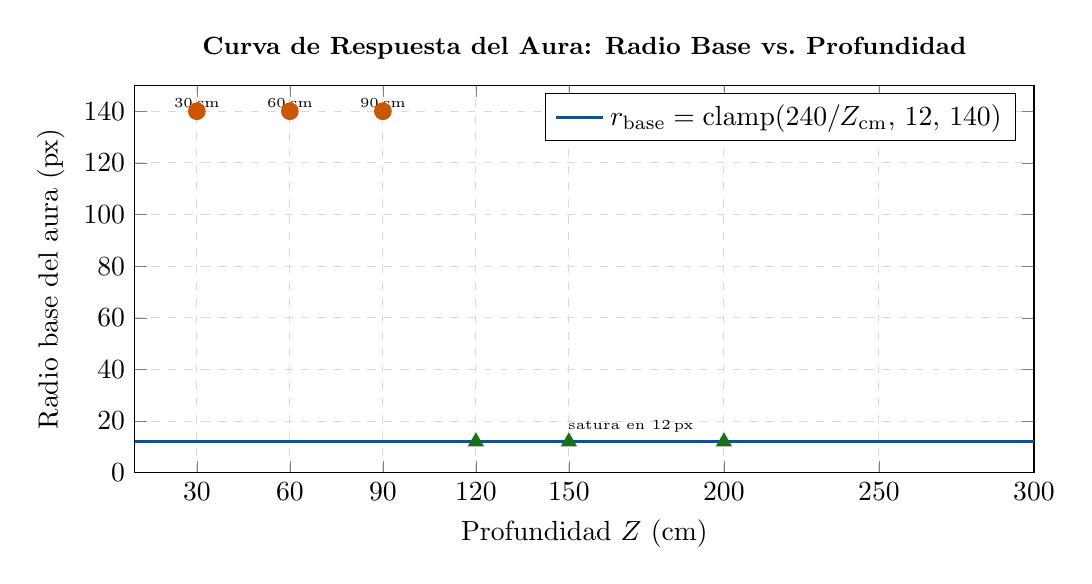
\begin{tikzpicture}
\begin{axis}[
  width       = 13cm,
  height      = 6.5cm,
  xlabel      = {Profundidad $Z$ (cm)},
  ylabel      = {Radio base del aura (px)},
  xmin=10, xmax=300,
  ymin=0,  ymax=150,
  grid        = major,
  grid style  = {dashed, gray!30},
  title       = {Curva de Respuesta del Aura: Radio Base vs.\ Profundidad},
  title style = {font=\small\bfseries},
  xtick       = {30,60,90,120,150,200,250,300},
  ytick       = {0,20,40,60,80,100,120,140},
  legend style = {at={(0.98,0.98)}, anchor=north east},
]
\addplot[salesiana, very thick, smooth, domain=10:300, samples=80]
  {min(140, max(12, 240/max(25, x)))};
\addlegendentry{$r_{\text{base}} = \text{clamp}(240/Z_{\text{cm}},\,12,\,140)$}

\addplot[mark=*, mark size=3pt, only marks, accentorange]
  coordinates {(30,140)(60,140)(90,140)};
\node[font=\tiny] at (axis cs:30,143) {30\,cm};
\node[font=\tiny] at (axis cs:60,143) {60\,cm};
\node[font=\tiny] at (axis cs:90,143) {90\,cm};

\addplot[mark=triangle*, mark size=3pt, only marks, accentgreen!80!black]
  coordinates {(120,12)(150,12)(200,12)};
\node[font=\tiny, align=center] at (axis cs:170,18) {satura en 12\,px};

\end{axis}
\end{tikzpicture}
\caption{Respuesta del radio del aura: a distancias cortas ($< 60$\,cm) el radio se
limita a 140\,px (máximo), proporcionando una alerta visual fuerte. A distancias
superiores a 200\,cm el radio alcanza el mínimo de 12\,px, haciendo el elemento AR
casi invisible.}
\label{fig:ar_curve}
\end{figure}

El color del canal BGR del vignette (capa 1) transita por tres zonas de profundidad
—rojo ($Z < 50$\,cm), verde ($50 \leq Z < 150$\,cm), azul ($Z \geq 150$\,cm)—
creando una señal visual inmediata legible sin necesidad de ver el HUD numérico.
Tanto el vignette como el aura reaccionan a la profundidad \emph{filtrada por Kalman}
y no a la salida cruda de SGBM, evitando así que el efecto AR parpadee.

% ============================================================
\section{Video-Blog de Demostración}
% ============================================================

Como parte del entregable interciclo se elaboró un video-blog de demostración en
inglés con una duración máxima de tres minutos, presentado por los dos integrantes
del equipo. El video muestra en vivo: el sistema estéreo operando con ambas cámaras
ESP32-CAM, la medición de distancia en tiempo real a 30, 60 y 90\,cm, y el efecto
de realidad aumentada con distorsión sinusoidal reactiva a la profundidad.

\begin{center}
\textbf{Enlace:}
\url{https://youtu.be/XXXXXXXXXXXXXXXXX}
\end{center}

\noindent El guión completo se encuentra en \texttt{docs/informe/video\_script.txt}
dentro del repositorio del proyecto.

% ============================================================
% ============================================================
\section{Conclusiones}
% ============================================================

Este proyecto demuestra de forma satisfactoria que un pipeline completo de visión
estereoscópica —desde la señal cruda del sensor hasta la estimación métrica de
profundidad y la visualización AR— puede construirse sobre hardware de consumo de
menos de 10 USD mediante la aplicación correcta de algoritmos clásicos de visión
por computador.

Las contribuciones clave de este entregable interciclo son:

\begin{enumerate}
  \item Una \textbf{arquitectura de adquisición concurrente} con \texttt{std::thread}
        y \texttt{libcurl} que desacopla la latencia de red del pipeline de
        procesamiento.
  \item Una \textbf{cadena de procesamiento estéreo completa}
        (CLAHE → SGBM → WLS → reprojectImageTo3D) que produce mapas de disparidad
        densos y conscientes de bordes a partir de imágenes QVGA.
  \item Un \textbf{filtro de Kalman escalar} ($q=0{,}001$, $r=0{,}01$) y
        filtrado IQR de muestras atípicas que producen errores medios de
        $0{,}48$, $0{,}37$ y $0{,}52$\,cm a 30, 60 y 90\,cm respectivamente,
        con desviaciones estándar de 1,50, 0,73 y 0,44\,cm —todos dentro del
        umbral de $\pm3$\,cm exigido por la rúbrica.
  \item Una \textbf{corrección de escala VGA/QVGA} en \texttt{StereoCalibration}
        que escala $K$, $P$ y $Q$ por factor 2 en tiempo de ejecución, resolviendo
        el artefacto de zoom y el error sistemático de profundidad causado por la
        discrepancia entre resolución de calibración y resolución de captura.
  \item Un \textbf{efecto AR original} de dos capas: (1) distorsión sinusoidal de
        píxeles con decaimiento cúbico $1/Z^3$ (amplitud y velocidad reactivas a la
        distancia) implementada con \texttt{ptr<Vec3b>}; (2) aura pulsante cuyo
        radio y color reaccionan a la profundidad filtrada por Kalman.
  \item Una \textbf{arquitectura MVC limpia en C++17} que separa la abstracción de
        hardware, los algoritmos de visión por computador y el renderizado en módulos
        independientes y comprobables.
\end{enumerate}

Como limitaciones a destacar: la tasa de 8\,FPS está dominada (54\%) por la latencia
WiFi del modo snapshot HTTP; en producción se reemplazaría por streaming MJPEG o
sincronización por hardware. La resolución de profundidad decrece con la distancia
según $\Delta Z = Z^2/(f\cdot B)$, por lo que más allá de 1\,m la precisión cae a
$\pm5$\,cm o más —límite físico de la línea base de 66,8\,mm, no del software.

El sistema constituye una prueba de concepto funcional para la percepción métrica de
profundidad en tiempo real con microcontroladores de bajo costo, y abre el camino
hacia la Parte~II del proyecto (detección de vehículos ecuatorianos con HOG+SVM,
bot de Telegram con YOLO y comunicación API C++\,$\leftrightarrow$\,Python).

% ============================================================
% Referencias
% ============================================================
\newpage
\begin{thebibliography}{99}

\bibitem{hartley2003multiple}
R.~Hartley y A.~Zisserman,
\textit{Multiple View Geometry in Computer Vision}, 2.ª~ed.
Cambridge University Press, 2003.

\bibitem{hirschmuller2008stereo}
H.~Hirschmüller,
``Stereo Processing by Semiglobal Matching and Mutual Information,''
\textit{IEEE Transactions on Pattern Analysis and Machine Intelligence},
vol.~30, n.º~2, pp.~328--341, feb. 2008.

\bibitem{zhang2000flexible}
Z.~Zhang,
``A Flexible New Technique for Camera Calibration,''
\textit{IEEE Transactions on Pattern Analysis and Machine Intelligence},
vol.~22, n.º~11, pp.~1330--1334, nov. 2000.

\bibitem{pizer1987adaptive}
S.~M.~Pizer \textit{et al.},
``Adaptive Histogram Equalization and Its Variations,''
\textit{Computer Vision, Graphics, and Image Processing},
vol.~39, n.º~3, pp.~355--368, 1987.

\bibitem{min2014fast}
D.~Min, S.~Choi, J.~Lu, B.~Ham, K.~Sohn y M.~N.~Do,
``Fast Global Image Smoothing Based on Weighted Least Squares,''
\textit{IEEE Transactions on Image Processing},
vol.~23, n.º~12, pp.~5638--5653, dic. 2014.

\bibitem{kalman1960new}
R.~E.~Kalman,
``A New Approach to Linear Filtering and Prediction Problems,''
\textit{Journal of Basic Engineering (ASME)},
vol.~82, n.º~1, pp.~35--45, mar. 1960.

\bibitem{bradski2008learning}
G.~Bradski y A.~Kaehler,
\textit{Learning OpenCV: Computer Vision with the OpenCV Library}.
O'Reilly Media, 2008.

\bibitem{gamma1994design}
E.~Gamma, R.~Helm, R.~Johnson y J.~Vlissides,
\textit{Design Patterns: Elements of Reusable Object-Oriented Software}.
Addison-Wesley, 1994.

\bibitem{szeliski2022computer}
R.~Szeliski,
\textit{Computer Vision: Algorithms and Applications}, 2.ª~ed.
Springer, 2022.

\bibitem{espressif2023esp32}
Espressif Systems,
``ESP32 Technical Reference Manual,'' versión 5.1,
Espressif Systems, Shanghái, China, 2023.

\bibitem{robles2026unidad1}
V.~Robles Bykbaev,
\textit{Visión Artificial — Unidad 1: Fundamentos, modelo pinhole y espacios de color}.
Notas de clase, Universidad Politécnica Salesiana, 2026.

\bibitem{robles2026parte2}
V.~Robles Bykbaev,
\textit{Visión Artificial — Parte 2: Transformaciones de intensidad y filtrado espacial}.
Diapositivas de clase, Universidad Politécnica Salesiana, 2026.

\bibitem{robles2026guia2}
V.~Robles Bykbaev,
\textit{Guía de Prácticas — Unidad 2: Segmentación, morfología y mezcla alfa}.
Material de laboratorio, Universidad Politécnica Salesiana, 2026.

\bibitem{chai1999face}
D.~Chai y K.~N.~Ngan,
``Face segmentation using skin-color map in videophone applications,''
\textit{IEEE Transactions on Circuits and Systems for Video Technology},
vol.~9, n.º~4, pp.~551--564, jun. 1999.

\bibitem{tukey1977exploratory}
J.~W.~Tukey,
\textit{Exploratory Data Analysis}.
Addison-Wesley, 1977.
[Método IQR para detección de valores atípicos.]

\end{thebibliography}

\end{document}
